\section{Learning Rate Schedules}
\subsection{Introduction}
Learning rate is arguably one of the most critical hyperparameters of a deep learning model. By default, the usual optimization method (Stochastic Gradient Descent) has a fixed rate of update, which is the learning rate we set. If the learning rate is too high, the model might miss the global minima, if it is too low, the model may never converge, and the training will take too long, as shown in the figure below.
\begin{figure}[!ht]
    \centering
    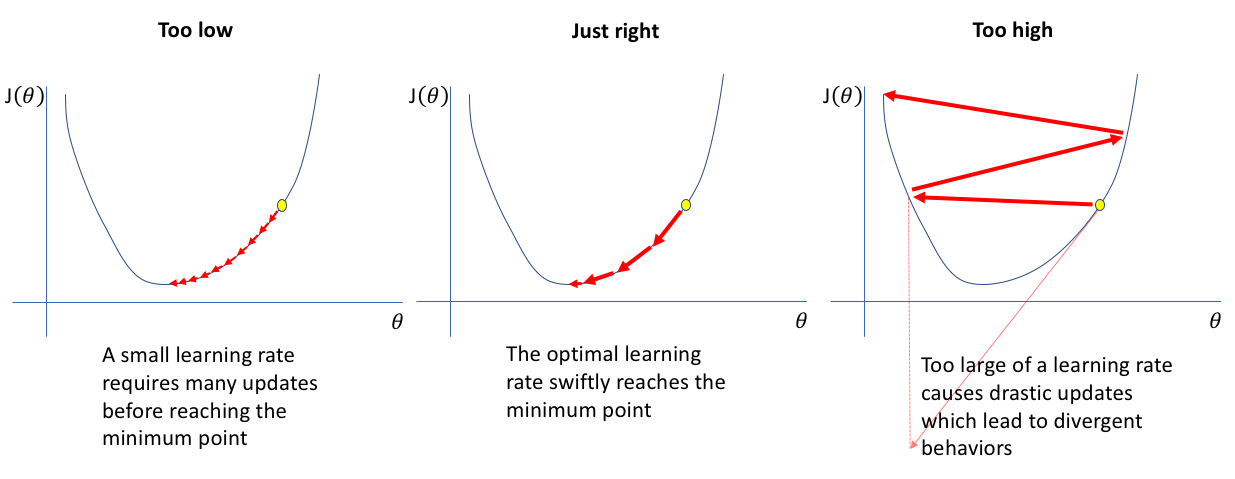
\includegraphics[scale=0.3]{./imgs/2019A7PS0097P-01.png}
    \caption{Learning rate example}
    \label{fig:learning_rate_ex}
\end{figure}


Researchers and practitioners alike have tried out an array of different methods to find out a way to arrive at the optimal learning rate, with the most prominent of them being the grid search. Even though a grid search may be successful in providing us with an optimal fixed learning rate, it still faces the problem of being fixed, i.e. not changing with the changes in our model. As shown in figure 1.1, ideally, our learning rate should take big steps when we are far from converging and smaller ones when we are close. This is tackled by having adaptive learning rates. As the name suggests, adaptive learning rates keep changing as our training goes on. How to change the learning rate is a question that has been explored by many different people in the field of deep learning, and as a result, we have multiple different methods to schedule our learning rate. We will be doing an analysis of these methods in the following sections.

\subsection{Learning Rate Schedules}
A smart schedule that varies the learning rate over time can result in much faster convergence and convergence to a better minimum than is possible otherwise. Large steps allow for a quick rise in the objective function, while smaller steps are required subsequently to descend into finer aspects of the loss landscape. Due to these properties, it has been observed in practice that using a learning rate scheduler results in not only a faster but also a better approximation of the minima. The most used variation of learning rate schedules is to gradually reduce the learning rate over time at each epoch. Effectively the process of scheduling learning rates can be broken down into two parts at a high level:
\begin{itemize}
    \item Early in the training phase, with a faster learning rate, choose a set of relatively "decent" weights.
    \item Later in the process, tune these weights to discover more ideal weights with a lower learning rate.
\end{itemize}
Further we will see some commonly used learning rate scheduling techniques, their advantages, drawbacks, and performance in some benchmark scenarios. As a baseline refer to the below figure of the performance of a ResNet50 architecture on the CIFAR10 dataset with a fixed learning rate of 0.1
\begin{figure}[!ht]
    \centering
    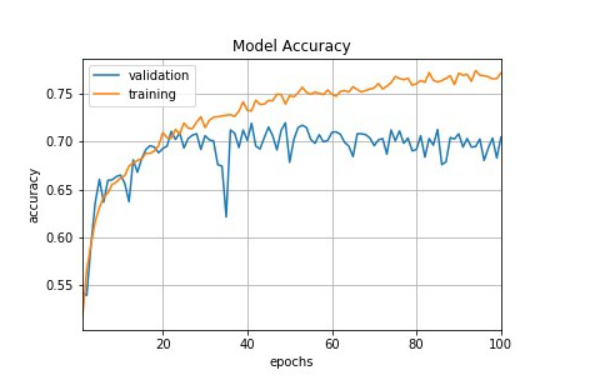
\includegraphics[scale=0.7]{./imgs/2019A7PS0097P-02.png}
    \caption{Constant Learning Rate}
    \label{fig:const_learn_rate}
\end{figure}

\subsection{Time based Decay}
Time based decay is one of the earliest forms of learning rate schedule. It introduces a factor of "decay", which decreases the learning rate by that factor after every epoch. The factor of decay is also a hyperparameter that is to be selected when training the model. Hence the new equation for the learning rate is dependent on the epoch that we are at and the decay selected by us. Below is the formula used for representing the learning rate.
\begin{center}
    \begin{math}
        lr = initial\_lr/(1+decay*(num\_of\_epoch*iterations\_per\_epoch))
    \end{math}
\end{center}

A convention to select the decay of the model is to set it to \(initial\_lr/num\_of\_epochs\), so for example, the initial learning rate is 0.1, and we want to train it for 100 epochs, our decay would be set to 0.01. We can plot the learning rate as a function of the epoch number, as shown in figure 1.3. The performance of this is actually a little worse than the constant lr method on the CIFAR-10 dataset. This shows us that learning rate schedules don't always work, but it does not mean that this method is altogether useless. With a different set of parameters, the result could have been different.
\begin{figure}[!ht]
  \centering
  \begin{minipage}[b]{0.4\textwidth}
    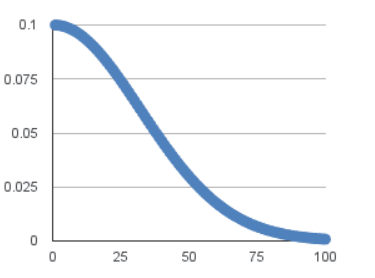
\includegraphics[width=\textwidth]{./imgs/2019A7PS0097P-03.png}
    \caption{Time based decay}
    \label{fig:time_based_decay}
  \end{minipage}
  \hfill
  \begin{minipage}[b]{0.4\textwidth}
    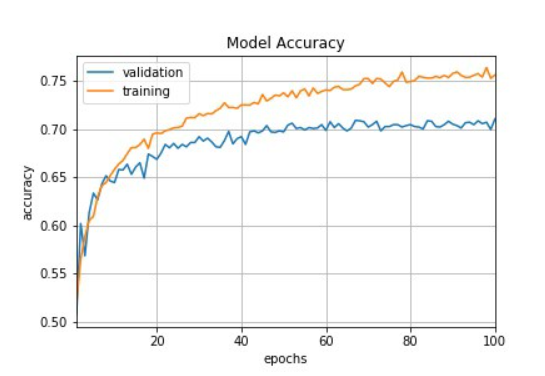
\includegraphics[width=\textwidth]{./imgs/2019A7PS0097P-04.png}
    \caption{Performance of Time based decay}
  \end{minipage}
\end{figure}


\subsection{Drop based Decay}
Unlike Time based decay which gradually decreases the learning rate every epoch, drop based decay drops the learning rate by a relatively large decay factor once every fixed number of epochs. 
This approach is frequently implemented by halving the learning rate after a set number of epochs. For example, we may start with a 0.1 learning rate and reduce it by 0.5 every 10 epochs. The first ten epochs of training would use a learning rate of 0.1, and the following ten epochs would use a learning rate of 0.05, and so on. The formula for drop based decay can be shown as:

\begin{center}
    \begin{math}
    lr = initial\_lr*drop\_factor^{(\lfloor                     num\_of\_epoch/drop\_epoch \rfloor)}
    \end{math}
\end{center}
We show the plot of the function in figure 1.5. A comparative study with the CIFAR-10 dataset is shown in figure 1.6, but with this method, we see a significant increase in the accuracy of our model (87\% from 84\%) by simply a slight tweak in the way our learning rate is calculated. Furthermore, both our training and validation losses are also dropping at the end of our training, showing affirmative results.
\begin{figure}[!ht]
  \centering
  \begin{minipage}[b]{0.4\textwidth}
    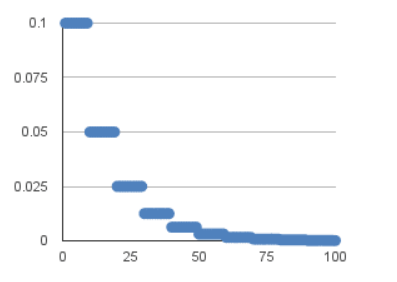
\includegraphics[width=\textwidth]{./imgs/2019A7PS0097P-05.png}
    \caption{Drop based decay}
    \label{fig:drop_based_decay}
  \end{minipage}
  \hfill
  \begin{minipage}[b]{0.4\textwidth}
    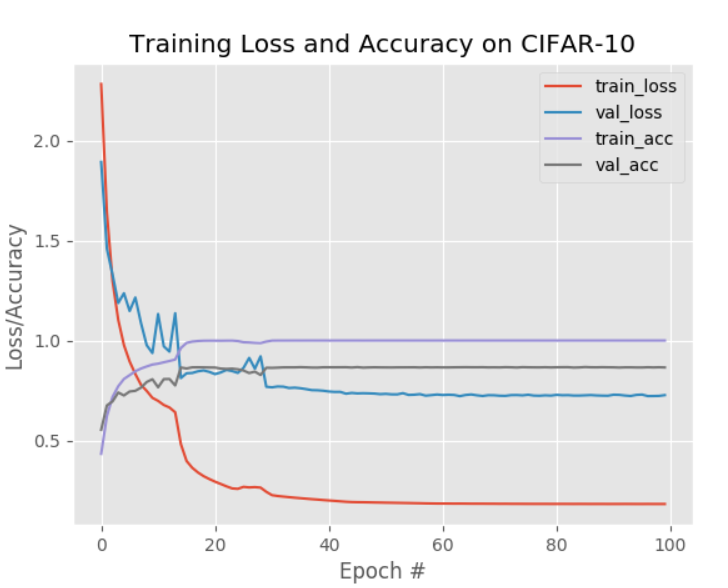
\includegraphics[width=\textwidth]{./imgs/2019A7PS0097P-06.png}
    \caption{Performance of Drop based decay}
  \end{minipage}
\end{figure}

As we can see that around the 15th to 20th epoch, the training and validation loss take a huge drop, and the accuracy takes a sharp increase. This is a characteristic feature of the drop based decay scheduling.

\subsection{Linear Decay} 
With this schedule, we linearly decrease the learning rate for each epoch. The linear decay starts off with the initial learning rate, and the rate is decreased gradually at each epoch till it is equal to 0 at the last epoch. The formula for linear decay is given below, and we can see from the formula that, unlike the previous methods we saw, the only hyperparameter we have to set is the initial learning rate. This method gives us the advantage that we don't need to do the selection for multiple hyperparameters with the learning rate.

\begin{center}
    \begin{math}
    lr = initial\_lr*(1-num\_of\_epoch/total\_epochs)
    \end{math}
\end{center}

The plot for linear decay is shown in figure 1.7. Running the same experiment on the CIFAR-10 dataset but this time with linear scheduling shows similar accuracy to our previous experiment (refer to figure 1.8), where we used drop based decay. This again shows how by simply using a learning rate scheduler, we saw a huge increase in the results from the baseline.

From figure 1.8, we can infer that, unlike the drop based decay method, the training loss decreases smoothly (although a steep drop is seen in the validation loss between epoch 70-80), and the accuracy too increases smoothly, with a decrease in the learning rate. Although basing our assumptions through just these two results would quite obviously be improper, experiments have shown a correlation between a decrease in learning rate as training goes on and better performance of the model in a positive sense.

\begin{figure}[!ht]
  \centering
  \begin{minipage}[b]{0.4\textwidth}
    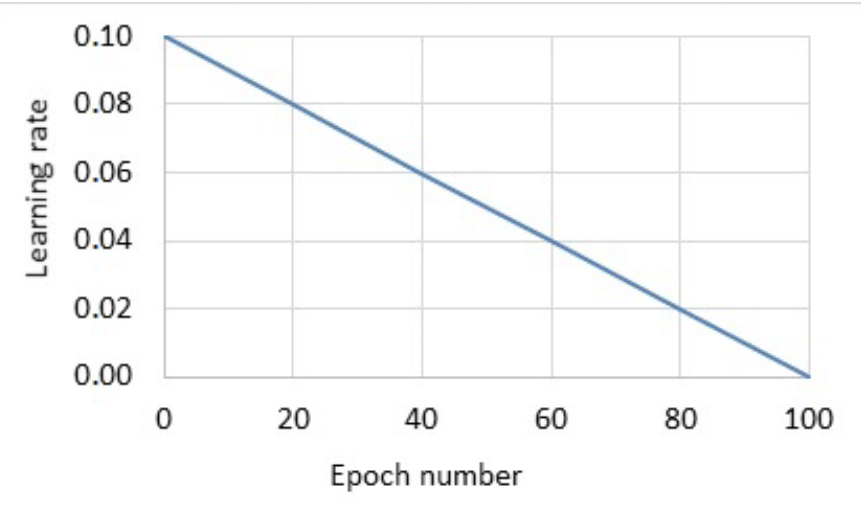
\includegraphics[width=\textwidth]{./imgs/2019A7PS0097P-08.png}
    \caption{Linear decay}
    \label{fig:linear_decay}
  \end{minipage}
  \hfill
  \begin{minipage}[b]{0.4\textwidth}
    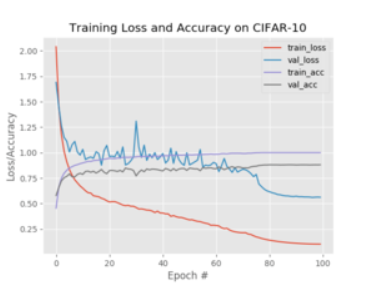
\includegraphics[width=\textwidth]{./imgs/2019A7PS0097P-07.png}
    \caption{Performance of Linear decay}
  \end{minipage}
\end{figure}
\newpage
\subsection{Polynomial Decay}
Polynomial decay can be obtained by a simple modification to the linear decay function. It can be seen as a general case of linear decay scheduling. We add a \(power\) factor to it, which basically determines the order of the decrease of the learning rate after each epoch. For the linear method, our \(power\) is set to 1.0 hence, making it linear, but if it was 2.0, our learning rate would have decreased quadratically and cubically for \(power\) equal to 3.0, and so on. 

\begin{center}
    \begin{math}
    lr = initial\_lr*(1-num\_of\_epoch/total\_epochs)^{power}
    \end{math}
\end{center}

This method introduces greater flexibility to our model by introducing another hyperparameter that we can fine-tune to obtain more desirable results. Below we show the plot for \(power=5.0\) in figure 1.9 for the function and the results obtained on the CIFAR-10 dataset in figure 1.10. We can see that we obtain similar results to drop based decay and linear decay, and we can see our training loss plateauing out after around 25 epochs.

\begin{figure}[!ht]
  \centering
  \begin{minipage}[b]{0.4\textwidth}
    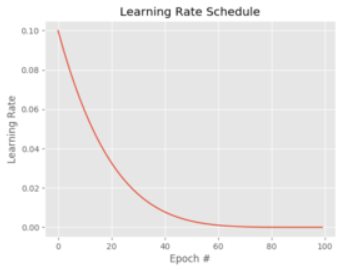
\includegraphics[width=\textwidth]{./imgs/2019A7PS0097P-09.png}
    \caption{Polynomial decay}
    \label{fig:polynomial_decay}
  \end{minipage}
  \hfill
  \begin{minipage}[b]{0.4\textwidth}
    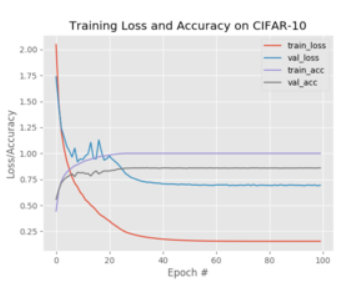
\includegraphics[width=\textwidth]{./imgs/2019A7PS0097P-10.png}
    \caption{Performance of Polynomial decay}
  \end{minipage}
\end{figure}

\subsection{Analysis}
\begin{table}[!ht]
    \centering
    \begin{tabular}{||c | c c c c c||}
         \hline Metric & Constant & Time based decay & Drop based decay & Linear decay & Polynomial decay \\ [0.5ex]
         \hline Accuracy & 0.84 & 0.82 & \textbf{0.87} & \textbf{0.87} & 0.86 \\
         \hline Loss & 0.5328 & 0.1732 & 0.1821 & \textbf{0.1040} & 0.1549 \\ [1ex]
         \hline
    \end{tabular}
    \caption{Result of using a ResNet model on the CIFAR-10 dataset with the corresponding learning rate schedules. Initial learning rate was 0.1 and trained for 100 epochs}
    \label{tab:my_label}
\end{table}

From the experiments conducted on the CIFAR-10 dataset \footnote{Learning rate schedules and decay using Keras}, we can see that the linear decay method performs the best and significantly better than the constant learning rate method. Although this in no way implies that only the linear decay method should be used for each task. Selecting the correct learning rate scheduling method is a very experimental process. The only way to know which schedule is best for your particular task is to actually run the model with different schedules. The results a certain schedule might give you depend on a lot of factors including, but not wholly on:
\begin{itemize}
    \item Initial learning rate
    \item Dataset being used
    \item Nature of the task
    \item The architecture being used
    \item Number of epochs during training
\end{itemize}

The learning rates that we discussed are the most common learning rates, but other scheduling methods are also used. Some of them are listed below
\begin{itemize}
    \item \subsubsection{Triangle Schedule}
    The triangle schedule involves using something called as \textit{warmup epochs} where you start with a very low learning rate or even 0, and gradually increase the learning rate to our "initial learning rate" and after reaching that point, use some kind of scheduling technique to again decrease the learning rate (linear warmup with linear decay is the most commonly used technique). This is usually used for training text classification models using BERT but could be tried for other tasks too.
    \item \subsubsection{Cosine Annealing}
    The cosine annealing schedule \footnote{Snapshot Ensembles: Train 1, get M for free, ICLR 2017} is an \textit{aggressive learning rate schedule}, in which the learning rate is initially large and then rapidly reduced to a low value around zero before being boosted to its maximum value. Its formula can be represented using the below formula. The equation takes as input the maximum learning rate that we want the model to reach, the number of cycles of oscillation that we want it to go through and the total number of epochs. Hence those are the hyperparameters for this method.
    \begin{center}
    \begin{math}
    lr(t)=\frac{maximum\_lr}{2}\left(\cos \left(\frac{\pi \bmod (num\_of\_epoch-1,\lceil total\_epochs / num\_of\_cycles\rceil)}{\lceil total\_epochs / num\_of\_cycles\rceil}\right)+1\right)
    \end{math}  
    \end{center}
    \begin{figure}[!ht]
  \centering
  \begin{minipage}[b]{0.4\textwidth}
    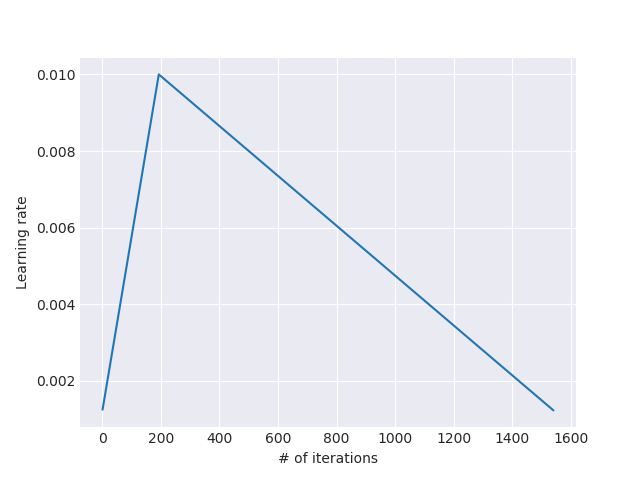
\includegraphics[width=\textwidth]{./imgs/2019A7PS0097P-11.jpg}
    \caption{Triangle Schedule}
    \label{fig:triangle_schedule}
  \end{minipage}
  \hfill
  \begin{minipage}[b]{0.4\textwidth}
    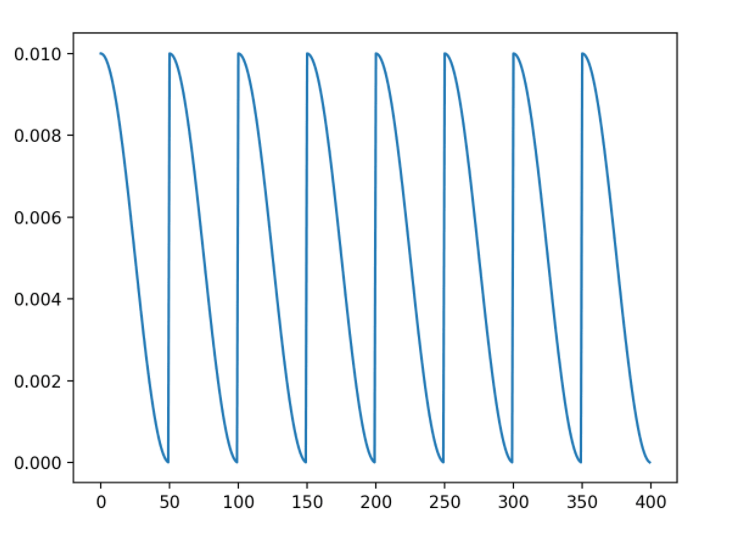
\includegraphics[width=\textwidth]{./imgs/2019A7PS0097P-12.png}
    \caption{Cosine Annealing}
  \end{minipage}
\end{figure}
\end{itemize}